% Options for packages loaded elsewhere
\PassOptionsToPackage{unicode}{hyperref}
\PassOptionsToPackage{hyphens}{url}
%
\documentclass[
]{book}
\usepackage{lmodern}
\usepackage{amssymb,amsmath}
\usepackage{ifxetex,ifluatex}
\ifnum 0\ifxetex 1\fi\ifluatex 1\fi=0 % if pdftex
  \usepackage[T1]{fontenc}
  \usepackage[utf8]{inputenc}
  \usepackage{textcomp} % provide euro and other symbols
\else % if luatex or xetex
  \usepackage{unicode-math}
  \defaultfontfeatures{Scale=MatchLowercase}
  \defaultfontfeatures[\rmfamily]{Ligatures=TeX,Scale=1}
\fi
% Use upquote if available, for straight quotes in verbatim environments
\IfFileExists{upquote.sty}{\usepackage{upquote}}{}
\IfFileExists{microtype.sty}{% use microtype if available
  \usepackage[]{microtype}
  \UseMicrotypeSet[protrusion]{basicmath} % disable protrusion for tt fonts
}{}
\makeatletter
\@ifundefined{KOMAClassName}{% if non-KOMA class
  \IfFileExists{parskip.sty}{%
    \usepackage{parskip}
  }{% else
    \setlength{\parindent}{0pt}
    \setlength{\parskip}{6pt plus 2pt minus 1pt}}
}{% if KOMA class
  \KOMAoptions{parskip=half}}
\makeatother
\usepackage{xcolor}
\IfFileExists{xurl.sty}{\usepackage{xurl}}{} % add URL line breaks if available
\IfFileExists{bookmark.sty}{\usepackage{bookmark}}{\usepackage{hyperref}}
\hypersetup{
  pdftitle={InspiRed Home Cooking},
  pdfauthor={Kate Nelson},
  hidelinks,
  pdfcreator={LaTeX via pandoc}}
\urlstyle{same} % disable monospaced font for URLs
\usepackage{longtable,booktabs}
% Correct order of tables after \paragraph or \subparagraph
\usepackage{etoolbox}
\makeatletter
\patchcmd\longtable{\par}{\if@noskipsec\mbox{}\fi\par}{}{}
\makeatother
% Allow footnotes in longtable head/foot
\IfFileExists{footnotehyper.sty}{\usepackage{footnotehyper}}{\usepackage{footnote}}
\makesavenoteenv{longtable}
\usepackage{graphicx,grffile}
\makeatletter
\def\maxwidth{\ifdim\Gin@nat@width>\linewidth\linewidth\else\Gin@nat@width\fi}
\def\maxheight{\ifdim\Gin@nat@height>\textheight\textheight\else\Gin@nat@height\fi}
\makeatother
% Scale images if necessary, so that they will not overflow the page
% margins by default, and it is still possible to overwrite the defaults
% using explicit options in \includegraphics[width, height, ...]{}
\setkeys{Gin}{width=\maxwidth,height=\maxheight,keepaspectratio}
% Set default figure placement to htbp
\makeatletter
\def\fps@figure{htbp}
\makeatother
\setlength{\emergencystretch}{3em} % prevent overfull lines
\providecommand{\tightlist}{%
  \setlength{\itemsep}{0pt}\setlength{\parskip}{0pt}}
\setcounter{secnumdepth}{5}
\usepackage{booktabs}
\usepackage{amsthm}
\makeatletter
\def\thm@space@setup{%
  \thm@preskip=8pt plus 2pt minus 4pt
  \thm@postskip=\thm@preskip
}
\makeatother
\usepackage[]{natbib}
\bibliographystyle{apalike}

\title{InspiRed Home Cooking}
\author{Kate Nelson}
\date{2020-11-25}

\begin{document}
\maketitle

{
\setcounter{tocdepth}{1}
\tableofcontents
}
\hypertarget{howdy}{%
\chapter*{Howdy}\label{howdy}}
\addcontentsline{toc}{chapter}{Howdy}

This is a cookbook made in R. Yes, a literal cookbook. Not one of those ``Cookbook for R'' types with ``recipes'' for R code to do fun stuff with data. This cookbook has recipes that you will actually want to whip up in your kitchen and consume to nourish your body. Why make this in R you ask. Why not? I enjoy R (it clearly has invaded all aspects of my life) and it was an amusing way to learn the \texttt{Bookdown} package.

\protect\hyperlink{botchien}{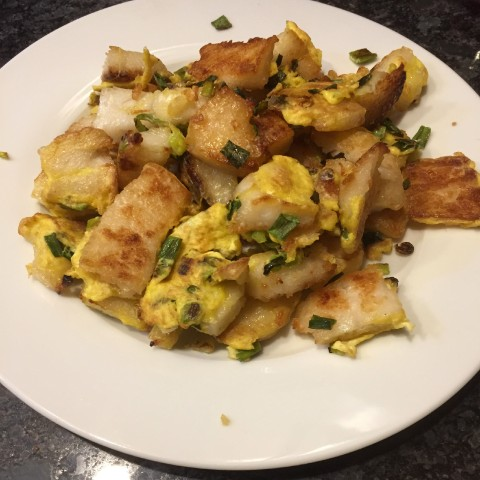
\includegraphics[width=1\textwidth,height=\textheight]{bot_chien_small.jpg}}
\protect\hyperlink{botchien}{Bot chien}

\protect\hyperlink{bohue}{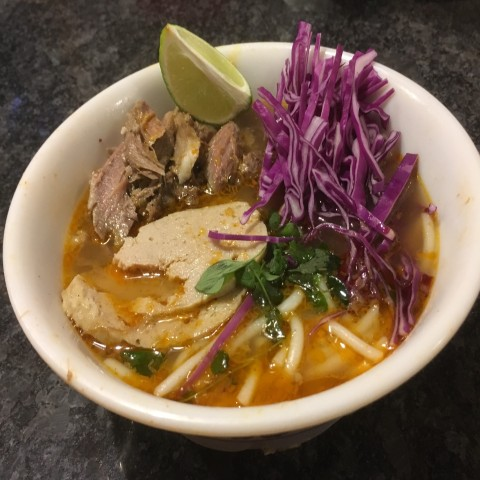
\includegraphics[width=1\textwidth,height=\textheight]{bun_bo_hue_small.jpg}}
\protect\hyperlink{bohue}{Bun bo hue}

\protect\hyperlink{burger}{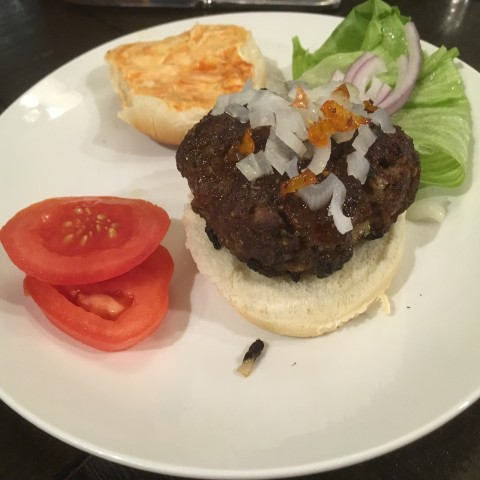
\includegraphics[width=1\textwidth,height=\textheight]{falafel_burger_small.jpg}}
\protect\hyperlink{burger}{Falafel Burger}

\protect\hyperlink{bbq}{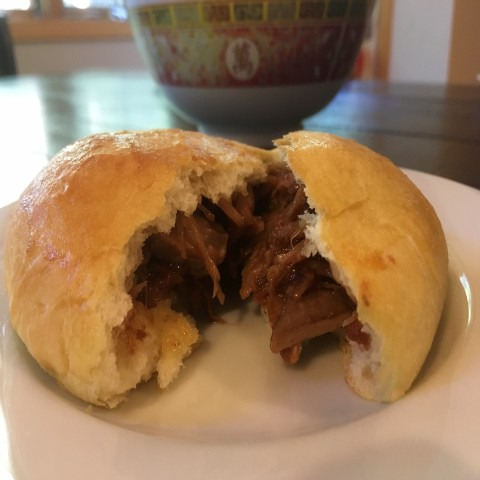
\includegraphics[width=1\textwidth,height=\textheight]{bbq_pork_buns_small.jpg}}
\protect\hyperlink{bbq}{BBQ pork buns}

\protect\hyperlink{hotchicken}{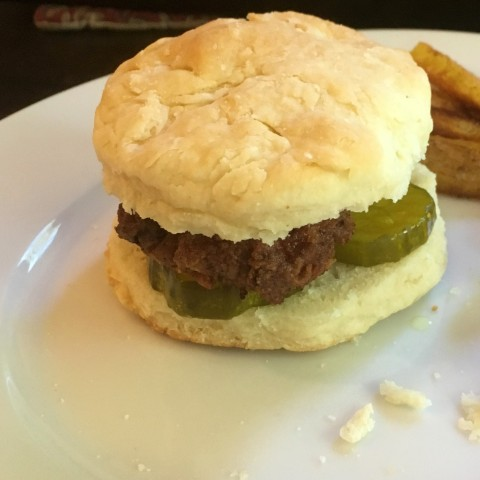
\includegraphics[width=1\textwidth,height=\textheight]{hot_chicken_small.jpg}}
\protect\hyperlink{hotchicken}{Hot Chicken}

\protect\hyperlink{hottofu}{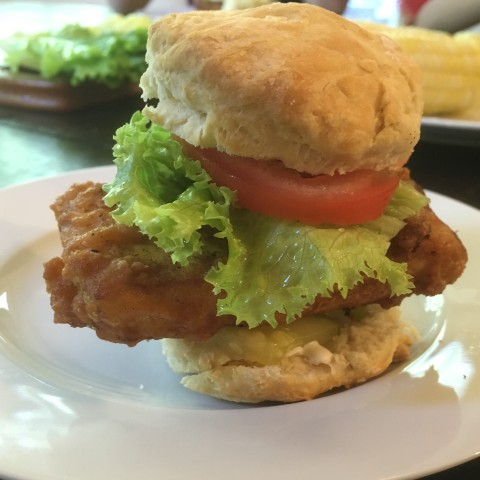
\includegraphics[width=1\textwidth,height=\textheight]{hot_chicken_tofu_small.jpg}}
\protect\hyperlink{hottofu}{Hot-chicken-fried tofu}

\protect\hyperlink{crustybread}{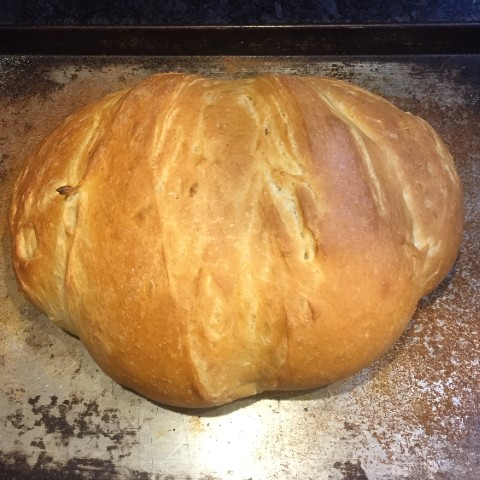
\includegraphics[width=1\textwidth,height=\textheight]{crusty_bread_small.jpg}}
\protect\hyperlink{crustybread}{Crusty bread}

\protect\hyperlink{moussaka}{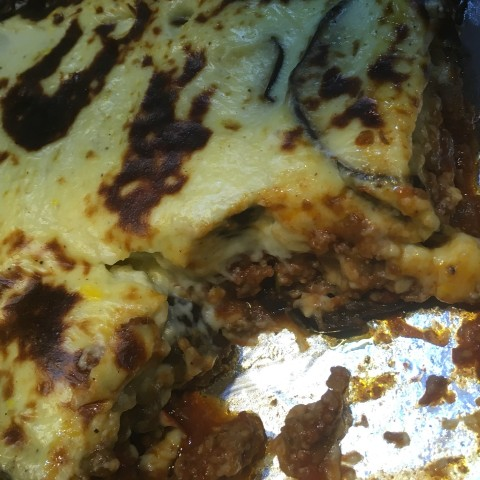
\includegraphics[width=1\textwidth,height=\textheight]{moussaka_small.jpg}}
\protect\hyperlink{moussaka}{Moussaka}

\protect\hyperlink{crispyrice}{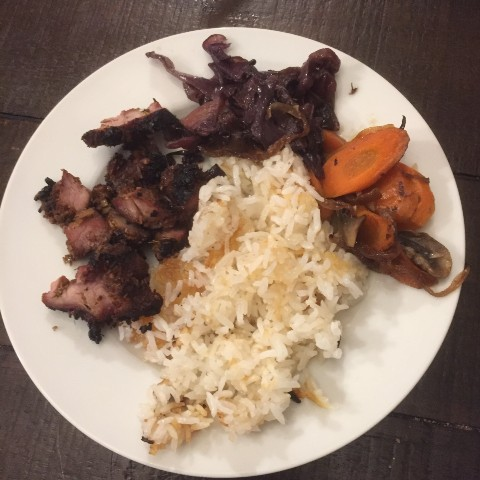
\includegraphics[width=1\textwidth,height=\textheight]{crispy_rice_small.jpg}}
\protect\hyperlink{crispyrice}{Crispy Rice}

\protect\hyperlink{gingerfish}{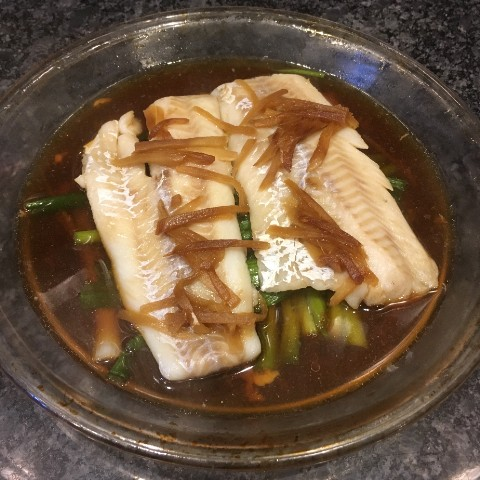
\includegraphics[width=1\textwidth,height=\textheight]{ginger_fish_small.jpg}}
\protect\hyperlink{gingerfish}{Ginger Fish}

\protect\hyperlink{pumpkincake}{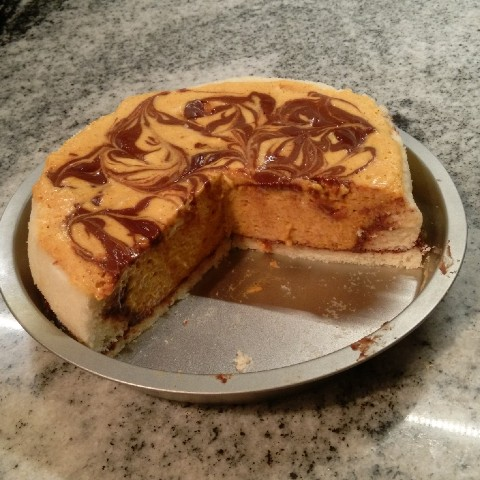
\includegraphics[width=1\textwidth,height=\textheight]{pumpkin_mousse_cake_small.jpg}}
\protect\hyperlink{pumpkincake}{Pumpkin Mousse Cake}

\protect\hyperlink{snailroll}{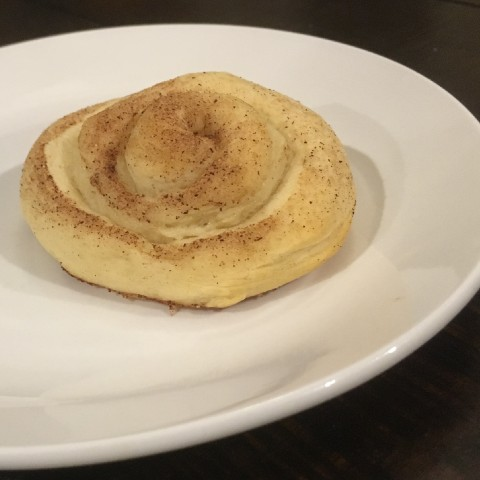
\includegraphics[width=1\textwidth,height=\textheight]{snail_roll_small.jpg}}
\protect\hyperlink{snailroll}{Snail Rolls}

\protect\hyperlink{cheesecake}{\includegraphics[width=1\textwidth,height=\textheight]{cheesecake.jpeg}}
\protect\hyperlink{cheesecake}{Creamy Cheesecake}

\hypertarget{viet}{%
\chapter*{Vietnamese}\label{viet}}
\addcontentsline{toc}{chapter}{Vietnamese}

This section is dedicated to Vietnamese recipes.

\hypertarget{soups}{%
\section*{Soups}\label{soups}}
\addcontentsline{toc}{section}{Soups}

\hypertarget{bohue}{%
\subsection*{Bun bo hue}\label{bohue}}
\addcontentsline{toc}{subsection}{Bun bo hue}

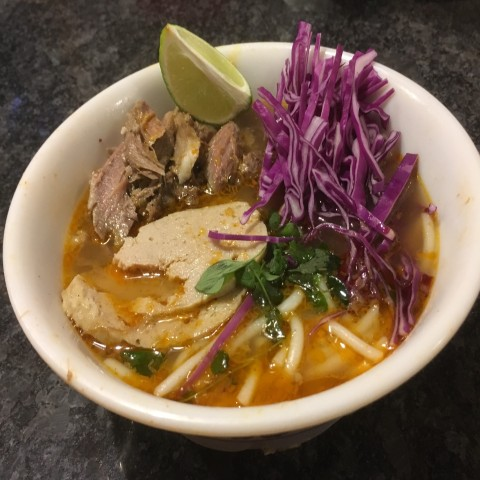
\includegraphics[width=0.4\textwidth,height=\textheight]{bun_bo_hue_small.jpg}

Bun bo hue is a wonderful alternative for those of you tired of pho. It includes both beef and pork in a sweet and savory broth flavored with pineapple, lemongrass, and shrimp paste. While it feels very meat indulgent this recipe easily provides 8 or more servings at \texttt{\textasciitilde{}1/2} pounds of meat (most of which is lower carbon footprint pork). The seasoning can be amped up a notch by adding a dollop of the spice mix to each bowl.

\begin{blackbox}

\textbf{Ingredients} (6-8 servings)

For the broth:

\begin{itemize}
\tightlist
\item
  1 large pork bone with some meat attached (or clean pork bones and 1/4 pound of pork shoulder)
\item
  1 large beef bone with some meat attached (or clean beef bones and 1/4 pound of chuck roast)
\item
  1 tbsp salt
\item
  1 tbsp sugar
\item
  1 can pineapple slices (with juice)
\item
  1 large yellow onion
\item
  4 stalks lemongrass or 1/8 cup chopped frozen lemongrass
\item
  8-10 cups water
\item
  2 tbsp shrimp paste
\item
  2 tbsp spice mix
\end{itemize}

For the spice mix:

\begin{itemize}
\tightlist
\item
  1/8 cup chopped lemongrass
\item
  1/8 cup minced shallots
\item
  2 tbsp minced garlic
\item
  1 tbsp annatto seeds
\item
  5 tbsp vegetable oil
\item
  1 package bun bo hue dry spice powder
\end{itemize}

For the soup:

\begin{itemize}
\tightlist
\item
  broth
\item
  spice mix
\item
  beef and pork from making broth (shredded)
\item
  vietnamese ham, sliced thin
\item
  2 packages bun bo hue noodles (thick rice noodles)
\item
  1/4 of a red cabbage, thinly sliced
\item
  wedge of lime
\item
  bunch of mint
\item
  bunch of thai basil, bean sprouts, sliced banana blossom (optional)
\end{itemize}

\end{blackbox}

\hypertarget{hutieu}{%
\subsection*{Hu tieu}\label{hutieu}}
\addcontentsline{toc}{subsection}{Hu tieu}

\textbf{\emph{Coming Soon}}

\hypertarget{noodles-and-rice}{%
\section*{Noodles and Rice}\label{noodles-and-rice}}
\addcontentsline{toc}{section}{Noodles and Rice}

\hypertarget{botchien}{%
\subsection*{Bot chien}\label{botchien}}
\addcontentsline{toc}{subsection}{Bot chien}

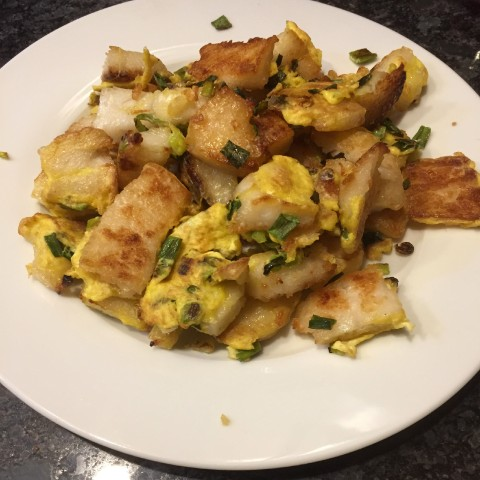
\includegraphics[width=0.4\textwidth,height=\textheight]{bot_chien_small.jpg}

Bot chien is a Vietnamese street food consisting of pan-fried rice cakes in a simple egg omelet. Traditionally pan-fried with LOTS of lard, we've worked up a lower grease recipe that still provides the wonderful crisp exterior and soft interior that makes this dish so craveable. This recipe is vegetarian, and is filling and satisfying enough that I've never once heard complaints about there not being any meat.

There are 3 components to this dish: the \textbf{rice cake}, the \textbf{omelet}, and the \textbf{sauce}. In many cities you can find pre-made rice (or taro, which works just as well) cakes at an Asian market. However, the rice cakes are simple to make from home if you can't buy them. You just need a large steamer and a heat safe dish that fits inside said steamer.

\begin{blackbox}

\textbf{Ingredients} (recipe serves 2-3 people)

For the rice cake:

\begin{itemize}
\tightlist
\item
  2 cup rice flour
\item
  2 tbsp tapioca starch
\item
  1 tbsp sugar
\item
  2 tsp oil
\item
  1 tsp salt
\end{itemize}

For the omelet:

\begin{itemize}
\tightlist
\item
  2-3 eggs
\item
  1/2 bunch green onions
\end{itemize}

For the sauce:

\begin{itemize}
\tightlist
\item
  1 cup soy sauce
\item
  1/2 cup sugar
\item
  1/2 cup white vinegar
\end{itemize}

\end{blackbox}

\begin{enumerate}
\def\labelenumi{\arabic{enumi}.}
\item
  To make the rice cake combine all ingredients in a large, heat-safe, microwavable bowl. Microwave for 2 minutes then carefully stir, scraping the sides of the bowl. Continue microwaving for \textasciitilde1 minute intervals, stirring afterwards, until mixture resembles slightly lumpy (and gummy) mashed potatoes.
\item
  While still warm gently press the mixture into a greased heat-safe casserole dish, Then place inside a large steamer and steam for \textasciitilde25 minutes until firm and a toothpick inserted in the center comes out mostly clean. (If doubling the recipe increase steaming time.)
\item
  Allow the rice cake to cool for at least a couple hours.\footnote{You can make these days in advance, but they do not freeze/thaw well so keep them in the fridge.}
\item
  While the rice cake is cooling make the sauce by heating the soy sauce, sugar and vinegar in a small sauce pan until the sugar dissolves and the mixture begins to bubble. Remove from the heat and allow to cool. (You can store this sauce at room temperature in a sterile glass jar.)
\item
  When the rice cake is cool cut it into \texttt{\textasciitilde{}\ 2\ inch\ X\ 2\ inch\ X\ 1/4\ inch} thick slices.
\item
  Beat the eggs and chop the green onions into small pieces.
\item
  Now it's time to pan-fry the rice cakes. This really needs to be done in small batches or the rice cakes won't crisp up. Heat a teaspoon of oil in a large non-stick skillet and add as many slices of rice cake as will comfortably fit in a single layer in your pan. Once the cakes begin to show a golden-carmel brown color on the bottom flip them over and add a handful of green onions and one more teaspoon of oil to the pan. Once the cakes are crisped on both sides add some of the beaten eggs and fry until the eggs are just cooked through.
\end{enumerate}

As a ``shortcut'', particularly if you plan on making this for more than 2 people, I recommend doing an initial cook of the rice cakes on large sheet pans in the oven. Liberally oil a large sheet pan, lay the rice cakes down in a single layer, then bake (use convection or ``air-fry'' mode if you have it) for 10-15 minutes per side at 525 degrees F. (The goal is to get the crisping started without drying the rice cake out.) You can then quickly finish the cakes with the green onion and egg in the skillet.

Serve the rice cakes with plenty of sauce drizzled over the top, some lime juice, and a bit of chili garlic sauce. Great with a side dish of \protect\hyperlink{cucsalad}{smashed cucumber salad}.

\hypertarget{banh}{%
\section*{Banh}\label{banh}}
\addcontentsline{toc}{section}{Banh}

\textbf{\emph{Coming Soon}}

\begin{itemize}
\item
  Banh Bao
\item
  Banh Xeo
\item
  Banh Mi
\end{itemize}

\hypertarget{meats}{%
\section*{Meats}\label{meats}}
\addcontentsline{toc}{section}{Meats}

\hypertarget{lgpork}{%
\subsection*{Lemongrass pork}\label{lgpork}}
\addcontentsline{toc}{subsection}{Lemongrass pork}

\textbf{\emph{Coming Soon}}

\hypertarget{extras}{%
\section*{Extras}\label{extras}}
\addcontentsline{toc}{section}{Extras}

\textbf{\emph{Coming Soon}}

\begin{itemize}
\item
  Pate
\item
  Pickled carrots and daikon
\item
  Eggrolls
\item
  Special fish sauce
\item
  Pickled mustard greens
\end{itemize}

\hypertarget{other-asian}{%
\chapter*{Other Asian}\label{other-asian}}
\addcontentsline{toc}{chapter}{Other Asian}

\hypertarget{chinese}{%
\section*{Chinese}\label{chinese}}
\addcontentsline{toc}{section}{Chinese}

\hypertarget{mapotofu}{%
\subsection*{Ma po tofu}\label{mapotofu}}
\addcontentsline{toc}{subsection}{Ma po tofu}

\textbf{\emph{Coming Soon}}

\hypertarget{gingerfish}{%
\subsection*{Ginger fish}\label{gingerfish}}
\addcontentsline{toc}{subsection}{Ginger fish}

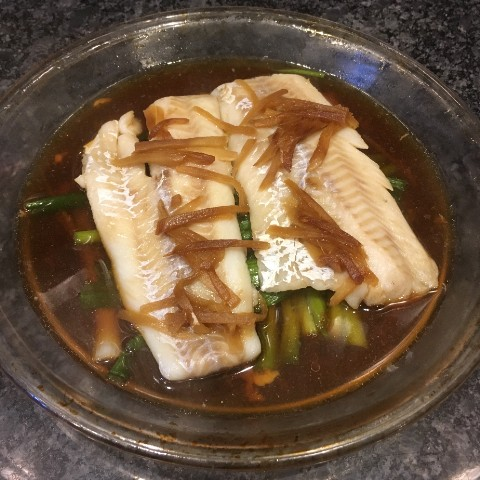
\includegraphics[width=0.4\textwidth,height=\textheight]{ginger_fish_small.jpg}

\hypertarget{cucsalad}{%
\subsection*{Smashed cucumber salad}\label{cucsalad}}
\addcontentsline{toc}{subsection}{Smashed cucumber salad}

\textbf{\emph{Coming Soon}}

\hypertarget{bbq}{%
\subsection*{BBQ Pork Buns}\label{bbq}}
\addcontentsline{toc}{subsection}{BBQ Pork Buns}

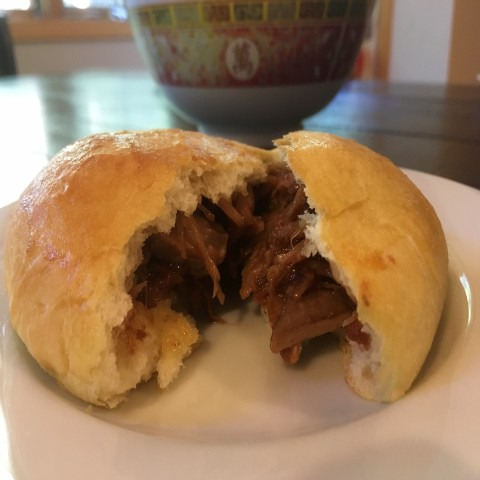
\includegraphics[width=0.4\textwidth,height=\textheight]{bbq_pork_buns_small.jpg}

Sauted bok choy in white sauce

Veggie Lo Mein

Rice noodle stir fry

Hot and sour soup

Egg drop soup

\hypertarget{japanese}{%
\section*{Japanese}\label{japanese}}
\addcontentsline{toc}{section}{Japanese}

Curry buns

White bean paste buns

Tatamen Spicy Ramen

Tonkatsu Pork Ramen

Miso

Fried Shrimp and Calamari Sushi

\hypertarget{korean}{%
\section*{Korean}\label{korean}}
\addcontentsline{toc}{section}{Korean}

\hypertarget{crispyrice}{%
\subsection*{Bibimbap with crispy rice}\label{crispyrice}}
\addcontentsline{toc}{subsection}{Bibimbap with crispy rice}

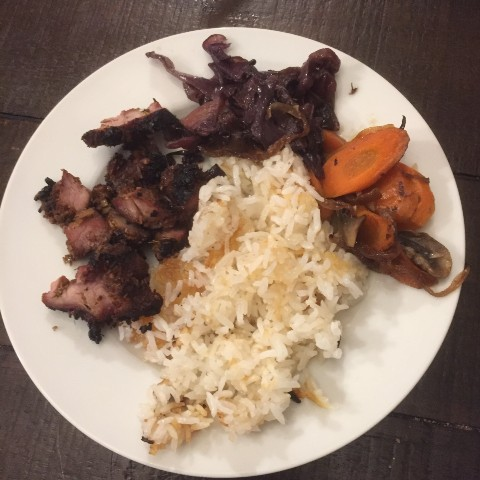
\includegraphics[width=0.4\textwidth,height=\textheight]{crispy_rice_small.jpg}

Jap chae

Leftover pancakes

\hypertarget{thai}{%
\section*{Thai}\label{thai}}
\addcontentsline{toc}{section}{Thai}

Coconut curry

Pad Thai

\hypertarget{other-savory-dishes}{%
\chapter*{Other Savory Dishes}\label{other-savory-dishes}}
\addcontentsline{toc}{chapter}{Other Savory Dishes}

\hypertarget{american}{%
\section*{American}\label{american}}
\addcontentsline{toc}{section}{American}

Ribs

\hypertarget{burger}{%
\subsection*{Falafel burgers}\label{burger}}
\addcontentsline{toc}{subsection}{Falafel burgers}

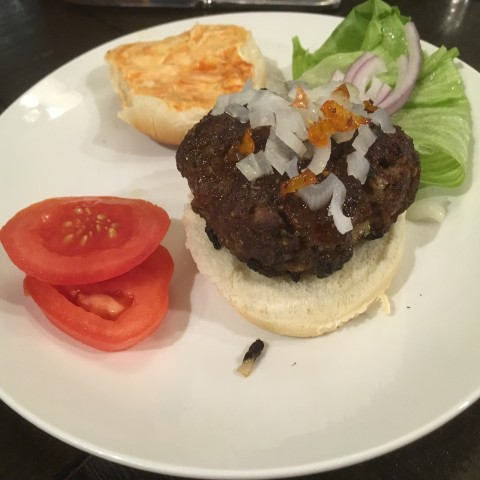
\includegraphics[width=0.4\textwidth,height=\textheight]{falafel_burger_small.jpg}

A wonderfull, juicy burger with half the meat.

\begin{blackbox}

\textbf{Ingredients} (4-5 servings)

\begin{itemize}
\tightlist
\item
  2/3 cup powdered falafel mix
\item
  1/4 cup water
\item
  1/2 onion
\item
  1/4 cup breadcrumbs
\item
  1 egg
\item
  1 lb ground beef
\end{itemize}

\end{blackbox}

\hypertarget{hotchicken}{%
\subsection*{Hot chicken}\label{hotchicken}}
\addcontentsline{toc}{subsection}{Hot chicken}

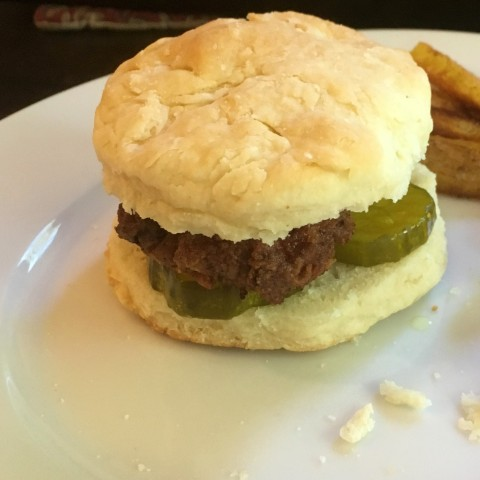
\includegraphics[width=0.4\textwidth,height=\textheight]{hot_chicken_small.jpg}

\hypertarget{hottofu}{%
\subsection*{Hot chicken-fried tofu}\label{hottofu}}
\addcontentsline{toc}{subsection}{Hot chicken-fried tofu}

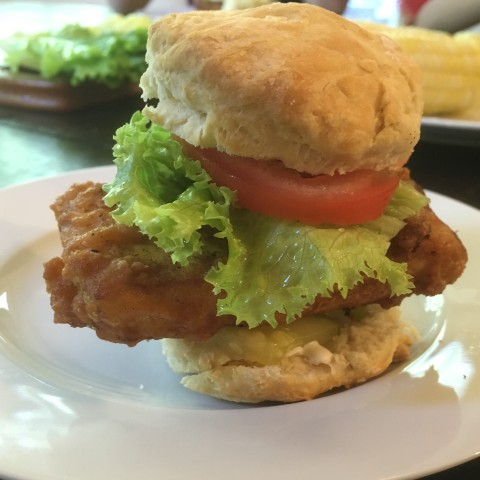
\includegraphics[width=0.4\textwidth,height=\textheight]{hot_chicken_tofu_small.jpg}

Home fries

Kale salad

Air-fried fish and chips

BBQ chicken pizza

Creamy tomato soup

Butternut squash mac and cheese

Pasta salad with olives

Biscuits and gravy

Corn chowder

Pulled meat

\hypertarget{indian}{%
\section*{Indian}\label{indian}}
\addcontentsline{toc}{section}{Indian}

Saag paneer

Sahi korma

Peas palag paneer

Pakoras

Tandori Chicken

Chicken korma

\hypertarget{european}{%
\section*{European}\label{european}}
\addcontentsline{toc}{section}{European}

\hypertarget{moussaka}{%
\subsection*{Moussaka}\label{moussaka}}
\addcontentsline{toc}{subsection}{Moussaka}

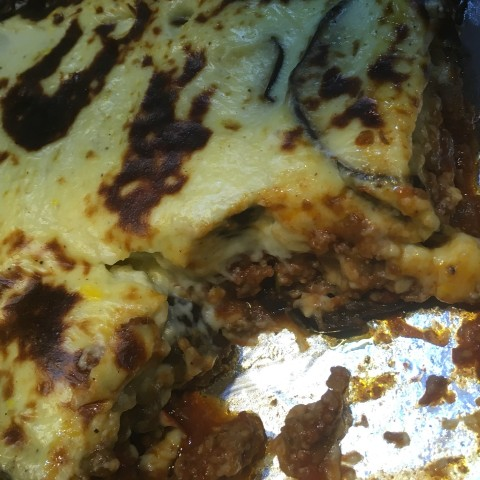
\includegraphics[width=0.4\textwidth,height=\textheight]{moussaka_small.jpg}

Spinach and beef lasagna

Pasta primavera

Gazpacho

Tabouli

Baba ganoush

Marinated tomatoes and cucumbers

Caldo Verde

Yorkshire Pudding with Beef and Mushrooms

\hypertarget{middle-eastern-and-african}{%
\section*{Middle Eastern and African}\label{middle-eastern-and-african}}
\addcontentsline{toc}{section}{Middle Eastern and African}

Kefta

Doro Wat

Kabobs

\hypertarget{latin-american}{%
\chapter*{Latin American}\label{latin-american}}
\addcontentsline{toc}{chapter}{Latin American}

Tamales

Papusas

Picadillo

\hypertarget{breads-and-desserts}{%
\chapter*{Breads and Desserts}\label{breads-and-desserts}}
\addcontentsline{toc}{chapter}{Breads and Desserts}

\hypertarget{bread}{%
\section*{Bread}\label{bread}}
\addcontentsline{toc}{section}{Bread}

\hypertarget{crustybread}{%
\subsection*{Crusty bread}\label{crustybread}}
\addcontentsline{toc}{subsection}{Crusty bread}

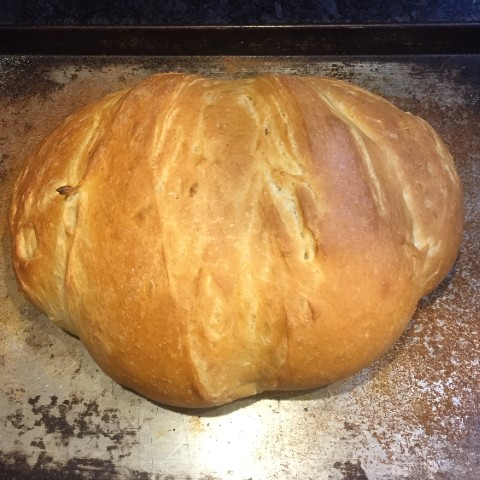
\includegraphics[width=0.4\textwidth,height=\textheight]{crusty_bread_small.jpg}

\hypertarget{snail-rolls-.unnumbered-snail-rolls}{%
\subsection{Snail Rolls \{.unnumbered \#snail rolls\}}\label{snail-rolls-.unnumbered-snail-rolls}}

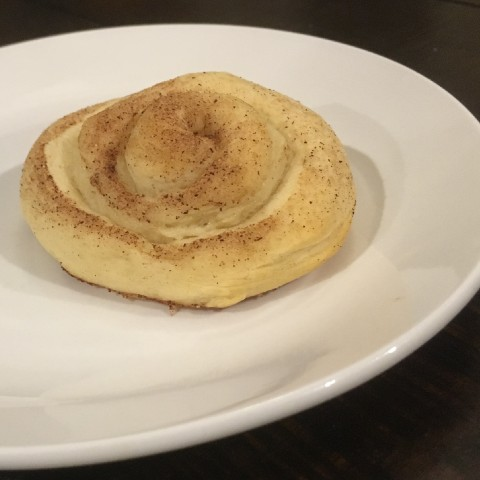
\includegraphics[width=0.4\textwidth,height=\textheight]{snail_roll_small.jpg}

A slightly sweet, low fat, milk bread roll. Great for breakfast or dessert.

\hypertarget{anpan}{%
\subsection*{An pan (milk bread for filled buns)}\label{anpan}}
\addcontentsline{toc}{subsection}{An pan (milk bread for filled buns)}

\hypertarget{monkey}{%
\subsection*{Monkey bread}\label{monkey}}
\addcontentsline{toc}{subsection}{Monkey bread}

Naan

Pizza dough

Beer bread

Dinner rolls

Donuts

French breakfast puffs

\hypertarget{desserts}{%
\section*{Desserts}\label{desserts}}
\addcontentsline{toc}{section}{Desserts}

\hypertarget{cheesecake}{%
\subsection*{Creamy cheesecake}\label{cheesecake}}
\addcontentsline{toc}{subsection}{Creamy cheesecake}

Delicious, creamy, cheesecake with more protien and less fat. 'Nough said.

\begin{blackbox}

\begin{itemize}
\tightlist
\item
  2 packages \textbf{greek} cream cheese \emph{(I find this has better flavor, texture, and mouthfeel than Neufatchel cheese and like it just as much, if not more than, full fat cream cheese.)}
\item
  1 cup heavy cream
\item
  1 cup sugar
\item
  3 eggs
\item
  1 tbsp vanilla
\item
  1/4 tsp salt
\end{itemize}

\end{blackbox}

Beat cream cheese and sugar until well mixed and cream cheese is soft and fluffy. Add eggs and salt and mix until fully incorporated. Add cream and vanilla and blend until smooth. Pour into a 12 inch nonstick springform pan with a prebaked shortbread or crumb crust. Bake at 300 for \textasciitilde45 minutes. Let cool completely before serving. Fantastic with warm rhubarb or plum compote.

\hypertarget{rhubarb-pie}{%
\subsection*{Rhubarb pie}\label{rhubarb-pie}}
\addcontentsline{toc}{subsection}{Rhubarb pie}

White bean paste buns

\hypertarget{pumpkincake}{%
\subsection*{Pumpkin mousse cake}\label{pumpkincake}}
\addcontentsline{toc}{subsection}{Pumpkin mousse cake}

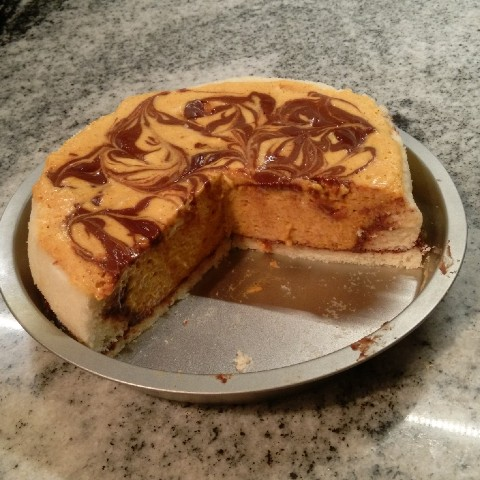
\includegraphics[width=0.4\textwidth,height=\textheight]{pumpkin_mousse_cake_small.jpg}

Crepes

Leftover jam

Leftover galletes

Lemon merengue pie

\hypertarget{delightful-leftovers}{%
\chapter*{Delightful Leftovers}\label{delightful-leftovers}}
\addcontentsline{toc}{chapter}{Delightful Leftovers}

Pulled meat

Lo mein

Bibimbap

Korean Pancakes

Fruit gallette

\hypertarget{lettuce-soup}{%
\subsection*{Lettuce soup}\label{lettuce-soup}}
\addcontentsline{toc}{subsection}{Lettuce soup}

Ever feel guilty about tossing that last bit of lettuce that's starting to brown, or isn't quite enough for a salad\ldots? I say unto you, ``lettuce eat soup''.
Ever

  \bibliography{book.bib,packages.bib}

\end{document}
